\begin{figure}
  \begin{center}
    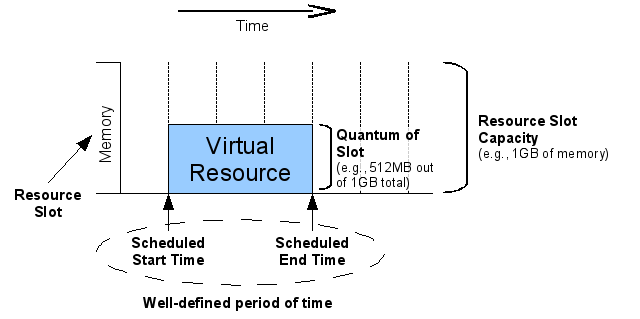
\includegraphics[width=0.8\textwidth]{figures/resourceslot.png}
    \caption{Resource Slot and Virtual Resource}
	\label{fig:resourceslot}
  \end{center}
\end{figure}

In this section, we present a resource management model that enables accurate and efficient creation and management of virtual workspaces in some of the resource management scenarios described in Section~\ref{cha:scenarios}, and which will allow us to tackle the problems described in the previous section. 

Our model assumes a set of physical resources providing a set of \emph{resource slots} (e.g., all the physical memory is one resource slot, each CPU is another resource slot, etc.). A quantum of a slot (e.g., 512 MB of memory, out of the 4 GB available) may be bound to a virtual workspace to provide it with some hardware resources needed to support the workspace's activities for a \emph{well{}-defined period of time}. We term such a binding of a portion of a slot to a virtual workspace a \emph{virtual resource}. All these concepts are summarized in Figure~\ref{fig:resourceslot}

Existing local resource managers, geared towards managing the execution of jobs, are not adequate for scheduling virtual resources because they would not take into account the overhead involved in deploying and managing those virtual resources. In particular, we encounter two types of overhead, which were alluded to in the previous section: \emph{preparation} and \emph{runtime}. The former refers to the cost of preparing the environment where the virtual workspace will run (most notably, deploying the VM images required by that workspace), while the latter refers to the memory, CPU and I/O overhead incurred by the VM hypervisor itself. Furthermore, these overheads are not necessarily constant, and may depend on the size of the requested virtual resources, the hypervisor used, and the quality of base resources.

Our model focuses on guaranteeing accuracy and maximizing efficiency. 
\begin{itemize}
\item[---] We define \emph{accuracy} as a binary property: a virtual workspace is either deployed accurately or not, without any gradients. Given a request to start a virtual workspace at time $t_s$ for a duration $d$, with resources $R$, the deployment is accurate if those conditions can be met. To accomplish this, we must account for preparation and runtime overhead in such a way that a request is only accepted if it can be guaranteed to be provisioned accurately since, otherwise, we would violate the agreement with the user requesting the workspace. This is distinct from the concept of \emph{fidelity} used by Irwin et al.\cite{BorjaCite10}, defined as the percentage of $d$ where the user has access to the resources (allowing for the actual starting time to be later than $t_s$, since part of $d$ could be consumed by preparation overhead in Irwin et al.'s work). Our model is designed to provide 100\% fidelity, rejecting any requests where this cannot be guaranteed. 
\item[---] We define \emph{efficiency} as a measure of how much we can reduce overhead, as opposed to making no attempt to manage it. Efficient processing of requests allows resources that would have otherwise been consumed by overhead to be used to process more requests. 
\end{itemize}

\begin{figure}
  \begin{center}
(a)

    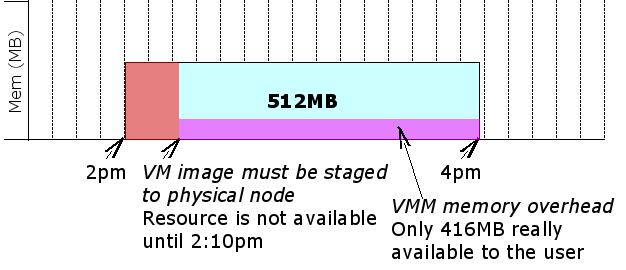
\includegraphics[width=0.8\textwidth]{figures/virtualresources_a.png}

\vspace{3em}
(b)

    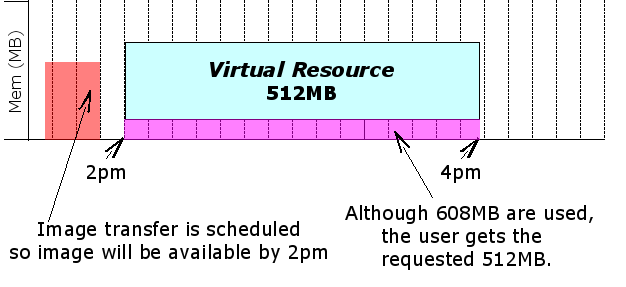
\includegraphics[width=0.8\textwidth]{figures/virtualresources_b.png}



    \caption{Virtual Resources and Overhead: (a) without considering overhead separately, and (b) considering overhead separately}
	\label{fig:virtualresources}
  \end{center}
\end{figure}

For example, let us assume that memory and time (availability) are the only two resources, and that a user requests 512MB of memory from 2pm to 4pm to support the execution of a workspace. Figure~\ref{fig:virtualresources}(a) shows how the resources allocated to the user would be diminished by two types of overhead: the preparation overhead of transferring the (potentially large) workspace's VM image to the physical node where it will run, delaying the start time of the workspace, and the runtime overhead of the virtual machine monitor. 

Using existing local resource managers, even those with AR capabilities, affects the accuracy of virtual workspace deployments, since they burden users with having to factor in the different types of overhead into their resource requests. This task is not easy because users cannot  predict the time to stage the VM image accurately, as they are unaware of the network traffic conditions on the site, and they have no control over how much of the virtual machine monitor's overhead will be deducted from their allocation (e.g., if several VM's are deployed on a single physical node, the deduction might be shared).

Thus, we argue in favor of a \emph{virtual resource management model}, where users get exactly the resources they requested. Thus, our model allows portions of resource slots to be bound either to virtual resources or
to overhead. The virtual resource accurately represents the resources requested by the user, and overhead is managed separately, instead of being deducted from the user's allocation. This separation results in more work for the local scheduler, which must now schedule both the virtual resource and the overhead, but results in increased accuracy and, as we will discuss in the following sections, enables the scheduler to take steps towards reducing overhead (increased efficiency).

For example, Figure~\ref{fig:virtualresources}(b) shows how a user's request for 512MB of memory from 2pm to 4pm is processed accurately by (1) \emph{scheduling} the preparation overhead of transferring the VM image (by prestaging it to the physical node before the scheduled start time of the virtual resource) and by (2) setting aside enough memory for the runtime overhead of the virtual machine without deducting it from the virtual resource.

Nonetheless, managing virtual resources and overhead involves challenges along several dimensions:

\begin{description}
\item[Time] (or \emph{availability}): We must guarantee that resources are available at the agreed--upon time, and must be able to reject requests that are deemed infeasible because it would not be possible to set up the required environment on time.
\item[Memory]: We must take into account that part of the memory in a physical node must be assigned to the virtual machine monitor. This dimension is trivial, since this memory usage is generally constant.
\item[Networking]: We must take into account that network bandwidth is shared by all the VMs on a physical node and with preparation overhead (such as image staging). Furthermore, network usage can affect CPU usage in the virtual machine monitor.
\item[Disk]: Similarly to networking, disk I/O is shared by all VMs on a node and can affect CPU usage in the virtual machine monitor. Furthermore, physical nodes must have enough disk space to support the VM images of different workspaces
\item[CPU]: The CPU share required by the virtual machine monitor can vary over time, depending on the resource usage of the VMs it is managing.
\end{description}

As mentioned in the introduction, we concern ourselves here with the resource dimension of availability, which is primarily affected by preparation overhead. In particular, workspace deployment can involve the (potentially expensive) transfer of a VM image to a node, a task that requires I/O and network usage that must be accounted for by the scheduler. However, we currently assume that VMs produce no network activity that would share bandwidth with preparation overhead (i.e. the Networking dimension does not affect the Time dimension).

The management of runtime overhead for the Xen virtual machine monitor was explored previously by Freeman et al. \cite{DBLP:conf/icsoc/FreemanKFRSW06}, and we leave an investigation of multi--dimensional scheduling of both preparation and runtime overhead for future work.
